\documentclass[11pt]{article}
\usepackage{classTools}

\begin{document}
% To include a problem set header, use the psHeader command
\psHeader{2}{Wed 2024-09-25 (11:59pm)}

\textbf{Your name: Nemeira Lal}

\textbf{Collaborators: Dani, Faseeh, Raphael}

\textbf{No. of late days used on previous psets: 1}

\textbf{No. of late days used after including this pset: 1}
\\

Please review the Syllabus for information on the collaboration 
policy, grading scale, revisions, and late days.

\begin{enumerate}
     \item  (designing reductions) 
     The purpose of this exercise is to give you practice designing reductions and proving their correctness and runtime.
    Consider the following computational problem:

    \compprob{AreaOfConvexPolygon()}
    {Points $(x_0,y_0),\ldots,(x_{n-1},y_{n-1})$ in the $\R^2$ plane that are the vertices of a convetx polygon (in an arbitrary order) whose interior contains the origin}
    {The area of the polygon formed by the points}


    \begin{enumerate}
        \item \label{part:polar} 
        Show that AreaOfConvexPolygon$\leq_{O(n),n}$ Sorting.  Be sure to analyze both the correctness and runtime of your reduction.

        In this part and the next one, you may assume that a point $(x,y)\in \R^2$ can be converted into polar coordinates $(r,\theta)$ in constant time. 
        \\\\
        You may find the following useful (and you may use them without proof):
        \begin{itemize}
            \item The polar coordinates $(r,\theta)$ of a point $(x,y)$ are the unique real numbers $r\geq 0$ and $\theta\in [0,2\pi)$ such that $x=r\cos \theta$ and $y=r\sin \theta$. Or, more geometrically, $r=\sqrt{x^2+y^2}$ is the distance of the point from the origin, and $\theta$ is the angle between the positive $x$-axis and the ray from the origin to the point.
            \item The area of a triangle is $A = \sqrt{s(s-a)(s-b)(s-c)}$ where $a, b, c$ are the side lengths of the triangle and $s = \frac{a + b + c}{2}$ (\href{https://en.wikipedia.org/wiki/Heron\%27s_formula}{Heron's Formula}).
        \end{itemize}
        The way to solve this is imagine all the vertices of the Polygon being points on a coordinate system. Next, the center is the (0,0) point. We can then break up this polygon as a set of triangles that connect adjacent vertices to the center, as shown in the diagram below. So, by finding the area of these individual triangles, we can add them all up to get the total area of the polygon. 
        \\ Furthermore, because it is not as easy to find the area given cartesian coordinates, we can convert all the points to polar and then use Heron's formula to find the area of the triangles based on their side lengths.
        \\ Let's break this up into a reduction problem, with all of the required steps and their runtimes:
        \begin{itemize}
            \item \textbf{Pre-processing:} Before we begin, we are given an array of Key-Value Pairs that signify the vertices of the polygons in cartesian coordinates. For our pre-processing, we want to convert this array into an array with polar coordinates of the polygon. However, we also want to preserve the cartesian coordinates of the vertices in our new array that we want to use, so we can find the length of the third side at a later point. So, our new array will contain the keys as the $\theta$, or the angle of the coordinate, and the value as a tuple $(r, (x,y))$. 
            \begin{itemize}
                \item \textbf{Runtime:} As we saw earlier, converting the cartesian to polar runs in $O(1)$ time, but we also have to go to every element of $n$, so, the total preprocessing time is $O(n)$.
            \end{itemize}

            \item \textbf{Oracle:} We sort the array that we created in the preprocessing step.
            \begin{itemize}
                \item \textbf{Runtime:} Becuase it is an oracle, we don't consider its runtime. So, just $O(1)$ because we call the oracle once.
            \end{itemize}

            \item \textbf{Post-processing:} First, we break our polygon into n different triangles that don't overlap, and then for each triangle, find the missing third side using their cartesian coordinates. Then, we find the area of each triangle using the two $r$ values of the polar points and the distance between the points through Heron's formula. Lastly, we add up the sums of the individual triangles to get the total area of the polygon.
            \begin{itemize}
                \item \textbf{Runtime:} Because each of these steps involve $O(1)$ runtime operations on $n$ different triangles, the runtime of this step should be $O(n)$
            \end{itemize}

            \item \textbf{Runtime Analysis:} Now that we have all the runtimes for the individual steps, let's combine them. The total runtime should be $O(n) + O(1) + O(n)$ = $\textbf{O(n)}$.

            \item \textbf{Proof of Correctness:} To compute the area of a convex polygon containing the origin, we break it into triangles formed by the origin and adjacent vertices. First, we convert the vertices into polar coordinates and sort them by their angles \(\theta\), ensuring that adjacent vertices in the sorted list correspond to adjacent vertices on the polygon. This sorting ensures that the triangles formed by consecutive vertices and the origin are non-overlapping. The area of each triangle is computed using Heron's formula, and summing the areas of these triangles gives the total area of the polygon. Convexity guarantees that all triangles fully cover the polygon without double-counting, ensuring that the computed area is correct.
        \end{itemize}
        \item Deduce that AreaOfConvexPolygon can be solved in time $O(n\log n)$.
        \\In the proof that we see above, we clearly ignored the oracle and its time complexity. However, using a sorting algorithm directly, specifically the Merge Sort, which is the fastest sort possible. Merge Sort has a run time of $O(n \cdot logn)$, and combining this with the pre-processing and post-processing steps, we get our final runtime to be:
        $$O(n) + O(n) + O(n \cdot logn) = O(n \cdot logn)$$
        
        \item (*challenge; extra credit; optional\footnote{This problem is meant to be done based on your enjoyment/interest and only if you have time. It won't make a difference between N, L, R-, and R grades (meaning it will only impact whether an R gets increased to an R+), and course staff will deprioritize questions about this problem at office hours and on Ed.})  Come up with a way to avoid conversion to polar coordinates and any other trigonometric functions in solving AreaOfConvexPolygon in time $O(n\log n)$.  Specifically, design an $O(n)$-time reduction that makes $O(1)$ calls to a Sorting oracle on arrays of length at most $n$, using only arithmetic operations $+$, $-$, $\times$, $\div$, and $\sqrt{\hspace{1em}}$, along with comparators like $<$ and $==$.  (Hint: first partition the input points according to which quadrant they belong in, and consider the slope of the line from a vertex (x,y) to the origin.) 
        \\\\ To avoid converting the coordinates into polar, we can take the slope approach instead. We currently use $\theta$ to sort the points and then find adjacent triangles. Instead, we can use the slopes of the points to do the same. 
        \\ However, we need to first divide the points into coordinates. That is because a positive slope may indicate a point in either quadrant 1 or quadrant 3, but we need a way to distinguish which quadrant a point is to be able to accurately find adjacent triangles.
        \\ So instead, we break each point into quadrants. Then, we sort them all based on their slopes. Lastly, we find the areas of adjacent triangles and add them all up. Let's write this formally:
        \begin{itemize}
            \item \textbf{Pre-Processing:} In this step, we divide each point into different quadrants. The way we do that is by comparing the signs on each:
            \begin{itemize}
                \item If $x > 0$ and $y > 0$: Quadrant 1
                \item If $x > 0$ and $y < 0$: Quadrant 2
                \item If $x < 0$ and $y < 0$: Quadrant 3
                \item If $x < 0$ and $y < 0$: Quadrant 4
                \item Then, we also compute the slope of each point using the formula $\frac{y}{x}$, and then put it in an array.
                \item \textbf{Runtime:} Because we are performing simple operations, the runtime of pre-processing is just O(n) for the n different points
            \end{itemize}

            \item \textbf{Oracle:} We sort the array that we created based on the slopes found in the preprocessing step.
            \begin{itemize}
                \item \textbf{Runtime:} Becuase it is an oracle, we don’t consider its runtime. So, just O(1) because we call the oracle once
            \end{itemize}
            \item \textbf{Post-processing:} Now that we know the adjacent vertices in the polygon, we can repeadetly use the distance formula, or $\sqrt{(x_2 - x_1)^2 + (y_2 - y_1)^2}$ between the two points and of the vertices from the origin themselves. Then, we can use Heron's formula using the three sides we formed. Lastly, we will add up all the individual areas of the triangles formed to get the final area of the triangle.
            \begin{itemize}
                \item \textbf{Runtime:} Again, because we are performing $O(1)$ operations on n elements, our runtime is simply $O(n)$
            \end{itemize}
            \item \textbf{Runtime Analysis:} So, our final runtime is:
            $$O(n) + O(1) + O(n) = O(n)$$
            
        \end{itemize}
        \label{part:nopolar}
        
\end{enumerate}
    
    Similar techniques to what you are using in this problem are used in algorithms for other important geometric problems, like finding the Convex Hull of a set of points, which has applications in graphics and machine learning.

    \item (composition of reductions) 
    The purpose of this exercise is to give you practice in working with the abstract definition of reductions.
    
    Let $\Pi, \Gamma, \Lambda$ be computational problems, and suppose that $\Pi\leq_{T_1(n),q_1(n)\times h_1(n)} \Gamma$ and $\Gamma \leq_{T_2(n),q_2(n)\times h_2(n)} \Lambda$, for non-decreasing functions $T_1,T_2,q_1,q_2,h_1,h_2$.  Determine functions $T_3,q_3,h_3$ in terms of $T_1,T_2,q_1,q_2,h_1,h_2$ such that 
    $$\Pi \leq_{O(T_3(n)),q_3(n)\times h_3(n)} \Lambda,$$
    and justify your answers. 
    (Hint: you can take $h_3(n)=h_2(h_1(n))$.)  
    \begin{itemize}
        \item \textbf{$T_3(n)$}: We can break it up into the two reductions that we see. Here, $\Pi$ is reduced to $\Gamma$, and $\Gamma$ is reduced to $\Lambda$. The runtime of the first reduction from $\Pi$ to $\Gamma$ is simply given by $T_1(n)$. As for the reduction from $\Gamma$ to $\Lambda$, we know that the runtime of the function is $T_2(n)$, but we also call $\Gamma$ exactly $q_1(n)$ times, and the size of the input is $h_1(n)$. So, the total runtime of the reduction from $\Gamma$ to $\Lambda$ is equal to $T_2(h_1(n))\cdot q_1(n)$. Hence, the total is:
    $$T_3(n) = T_1(n) + T_2(h_1(n))\cdot q_1(n)$$

        \item \textbf{$q_3(n):$} This number just denotes the number of times we call the oracle for $\Lambda$ while we are solving problem $\Pi$. First of all, we call $\Gamma$ exactly $q_1(n)$ times. For each of those calls to the oracle, we call $\Lambda$ exactly $q_2(n)$ times. Then, for each of those calls, the size of our input is $h_1(n)$. So, the total times we call the oracle is:
        $$q_3(n) = q_1(n) \cdot q_2(h_1(n))$$

        \item \textbf{$h_3(n):$} This is the total size of our input that we plug into $\Lambda$. First of all, the input in our first step from $\Pi$ to $\Gamma$ is $h_1(n)$. Then, we plug in that size into our second reduction component from $\Gamma$ to $\Lambda$, so that would be $h_2(h_1(n))$. So, in terms of $h_1(n)$ and $h_2(n)$,
        $$h_3(n) = h_2(h_1(n))$$
    \end{itemize}

    
    \item (augmented binary search trees) The purpose of this problem is to give you experience reasoning about correctness and efficiency of dynamic data-structure operations, on variants of binary-search trees. 
    
    Specifically, we will work with {\em selection data structures}.
    We have seen how binary search trees can support min queries in time $O(h)$, where $h$ is the height of the tree.  A generalization is {\em selection} queries, where given a natural number $q$, we want to return the $q$'th smallest element of the set.  So $\texttt{DS.select(0)}$ should return the key-value pair with the minimum key among those stored by the data structure $\texttt{DS}$, $\texttt{DS.select(1)}$ should return the one with the second-smallest key, $\texttt{DS.select(n-1)}$ should return the one with the maximum key if the set is of size $n$, and $\texttt{DS.select((n-1)/2)}$ should return the median element if $n$ is odd.
    
    In the Roughgarden text (\S11.3.9), it is shown that if we {\em augment} binary search trees by adding to each node $v$ the size of the subtree rooted at $v$, then Selection queries can be answered in time $O(h)$.\footnote{Note that the Roughgarden text uses a different indexing than us for the inputs to Select. For Roughgarden, the minimum key is selected by Select(1), whereas for us it is selected by Select(0).}
    
    \begin{enumerate}
        \item In the Github repository, we have given you a Python implementation of size-augmented BSTs supporting search, insertion, and selection, and with a stub for \texttt{rotate}. One of the implemented functions (\texttt{search}, \texttt{insert}, or \texttt{select}) has a correctness error, another one is too slow (running in time that's (at least) linear in the number of nodes of the tree rather than linear in the height of tree), and the third is correct. 

        Identify and correct these errors. You should provide a text explanation of the errors and your corrections, as well as implement the corrections in Python.

        \begin{itemize}
            \item \textbf{Search:} This is implemented correctly!
            \item \textbf{Select:} Correctness Error
            \begin{itemize}
                \item \textbf{Error:} If select runs correctly, it should return the ind\textit{th} node's tree. However, in the algorithm in the code, when we fail to find the ind\textit{th} node on the left, we move to check for that in the right. We return $self.right.select(ind)$, but we don't consider that ind is actually related to the entire size of the tree, and may as well be larger than the size of the right tree. 
                \\ \textbf{Correction:} To fix the issue, all we need to do is return the ind-left size-1\textit{th} element, because we have already looked and ignored the left side. So, then, we return $self.right.select(ind-left size-1)$ instead of $self.right.select(ind)$.
            \end{itemize}
            \item \textbf{Insert:} This algorithm is too slow, and is $O(n)$ instead of $O(h)$, which it can be
            \begin{itemize}
                \item \textbf{Error:} Right now, we calculate the size of the tree at the end of the insertion call. So, the calculate-sizes recursively checks through each and every node and updates the sizes to the new one. This makes the runtime $O(n)$ and not $O(h)$.
                \item \textbf{Correction:} To fix this mistake, all you need to do is calculate the size of the right or left subtree right after a new node is inserted.
            \end{itemize}
        \end{itemize}
        
        \item Describe (in pseudocode or pictures) how to extend \texttt{rotate} to size-augmented BSTs, and argue that your extension maintains the runtime $O(1)$. Prove that your new rotation operation preserves the invariant of correct size-augmentations. (That is, if every node's size attribute had the correct subtree size before the operation, then the same is true after the operation.)
        \\\\ 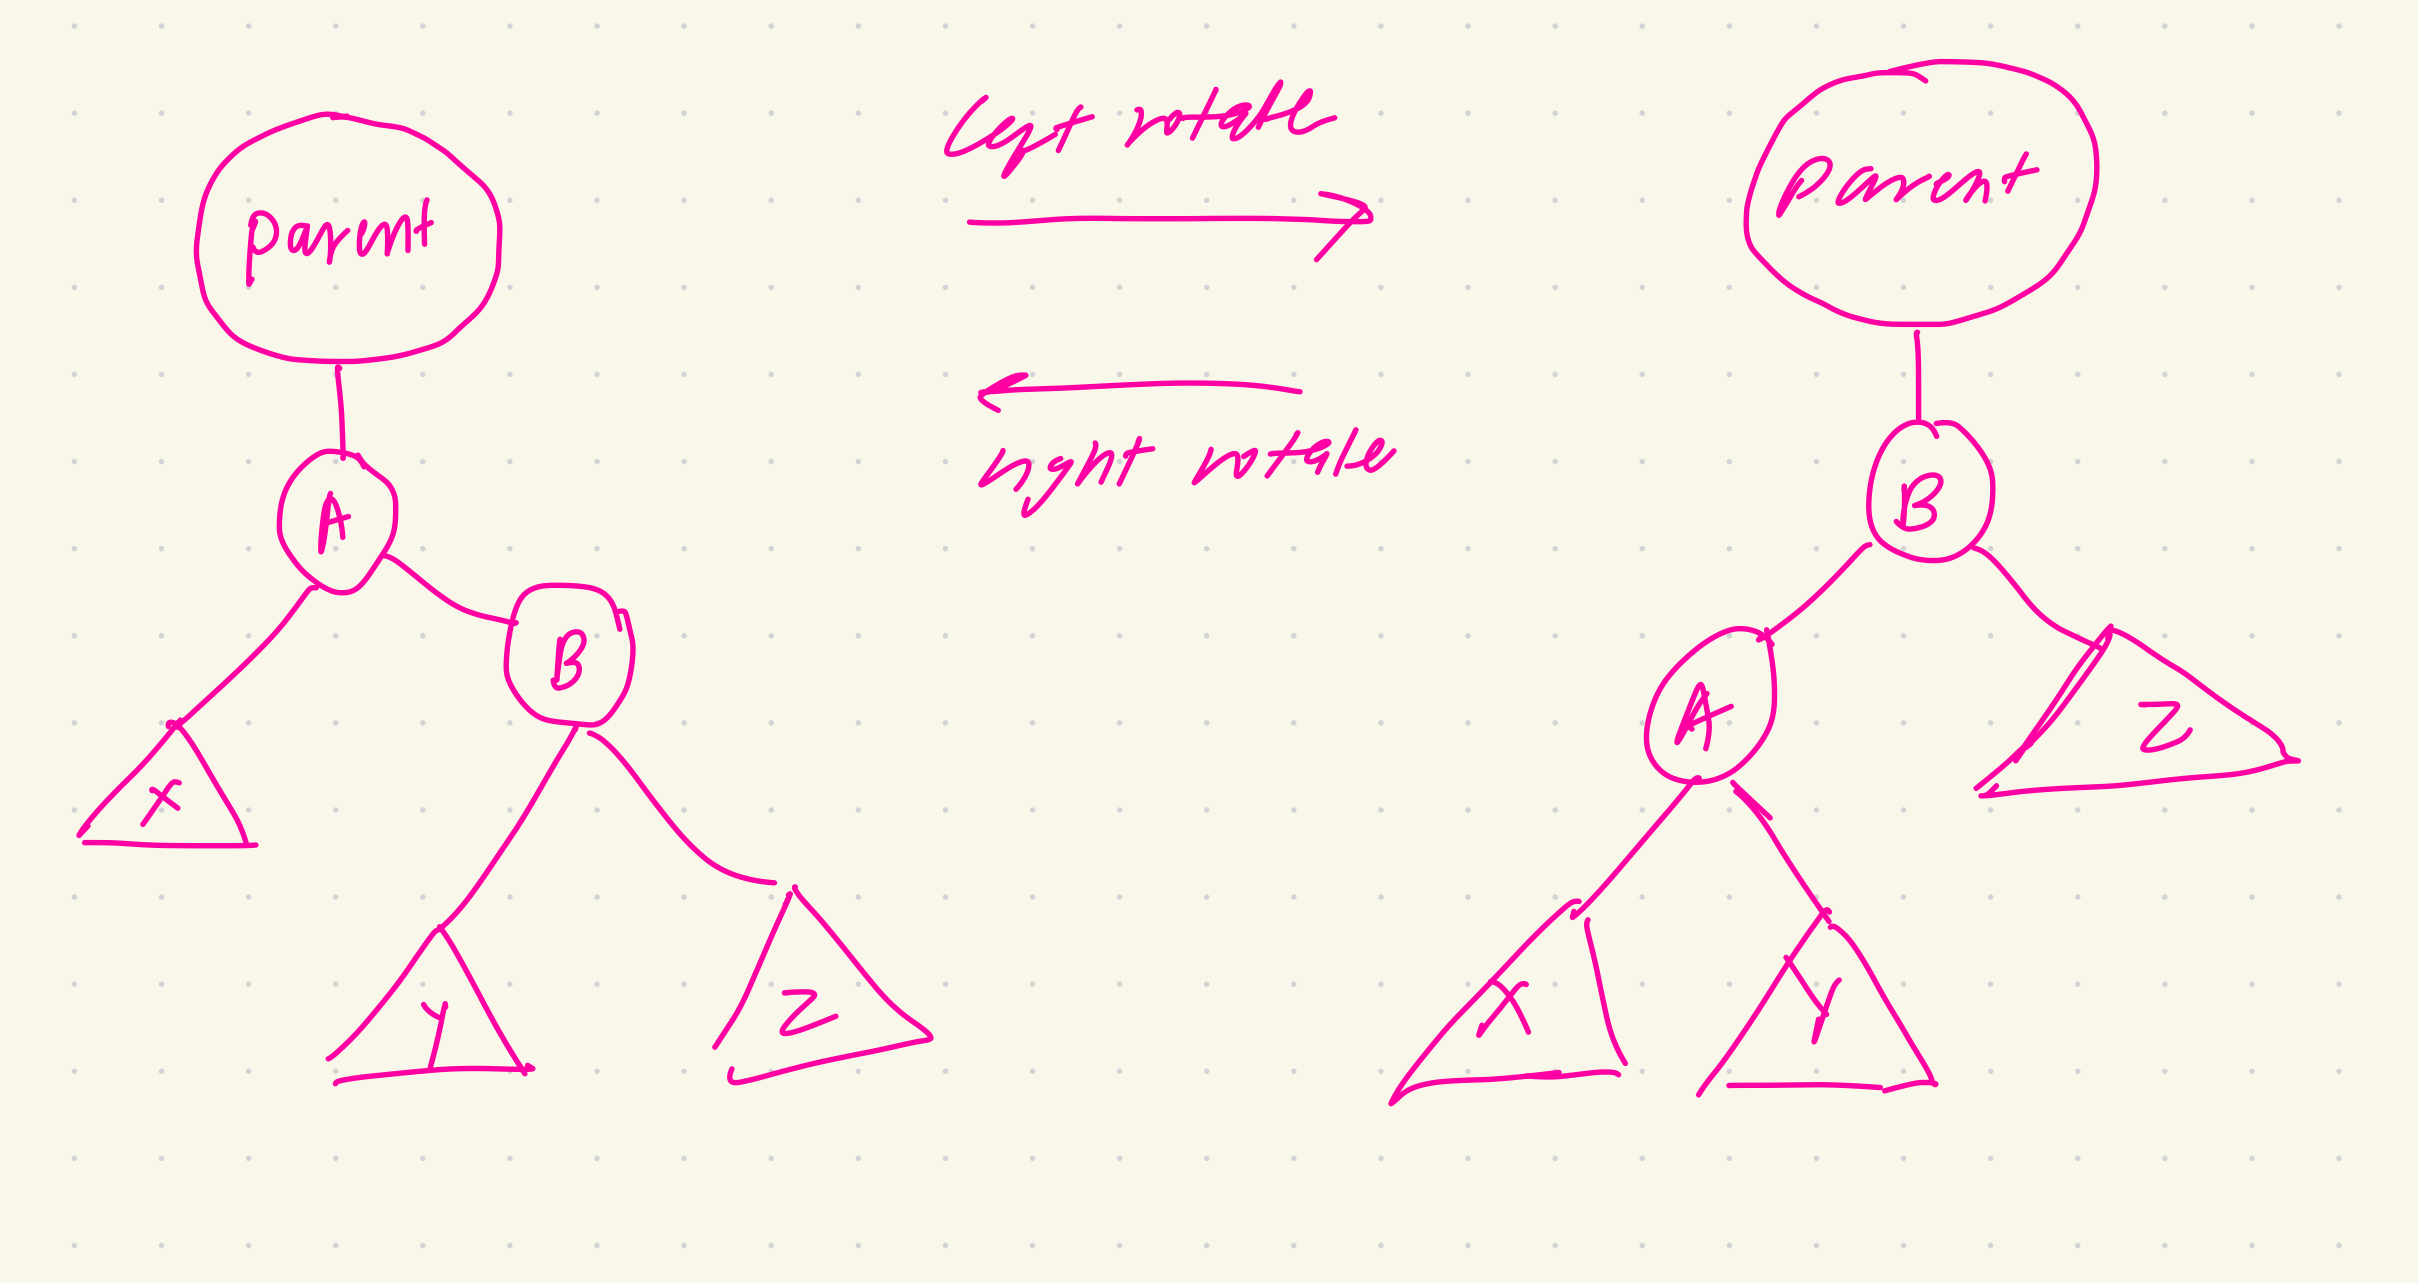
\includegraphics[scale = 0.1]{IMG_0130.jpg}
        \\Because we are just applying Rotate to size-augmented BSTs, we just need to make sure that the size of each node is correctly updated after the rotation. Focusing just on the left rotation operation, we only need to update the sizes of $A$ and $B$. Before, the size of A was just 1 + the sizes of its left and right subtrees, x and B. Similarly, the size of B was just the size of it's two subtrees, y and z. After the rotation, the size of A becomes 1 + size(x) + size(y), while the size of y becomes 1 + size(A) + size(z). All we need to do for rotate is just update the new sizes.
        \\ \textbf{Runtime:} The runtime is simply O(1) because we are only looking up the sizes of the subtrees and do a few arithmetic operations alongside.
        \\ \textbf{Correctness:} Assuming that the size attributes of all nodes were correct before the rotation, the correctness of the rotation is preserved after the operation. This is because we are recalculating the sizes of $A$ and $B$ based on their updated subtrees, using the correct sizes from before the rotation. As a result, the size invariants are maintained, ensuring that the size attributes remain correct. 
        
        \item Implement \texttt{rotate} in size-augmented BSTs in Python in the stub we have given you.
    
    \end{enumerate}
    
    \emph{Food for thought (do read - it's an important take-away from this problem):} This problem concerns size-augmented binary search trees. In lecture, we discussed AVL trees, which are balanced binary search trees where every vertex contains an additional \textit{height} attribute containing the length of the longest path from the vertex to a leaf (height-augmented). Additionally, every pair of siblings in the tree have heights differing by at most 1, so the tree is height-balanced. Note that if we augment a binary search tree both by size (as in the above problem) and by height (and use it to maintain the AVL property), then we create a dynamic data structure able to perform \texttt{search}, \texttt{insert}, and \texttt{select} all in time $O(\log n)$. 


\item (reflection) We aim for cs1200 to be a collaborative learning community. Describe two concrete ways in which you have supported, or will try to support, your classmates' learning in the course.  Be specific, connecting your answer to the structure of cs1200. 

\textit{Note: As with the previous psets, you may include your answer in your PDF submission, but the answer should ultimately go into a separate Gradescope submission form.}

\item Once you're done with this problem set, please fill out \href{https://forms.gle/pyhGJ73HpodhThNP9}{this survey} so that we can gather students' thoughts on the problem set, and the class in general. It's not required, but we really appreciate all responses!

\end{enumerate}



\end{document}
